\documentclass[a4paper,12pt]{article}
\usepackage[T2A]{fontenc}
\usepackage[utf8]{inputenc}
\usepackage[english,russian]{babel}
\usepackage{graphicx}
\usepackage{geometry}
\geometry{top=2cm,bottom=2cm,left=2.5cm,right=1.5cm}
\usepackage{float}
\usepackage{hyperref}
\usepackage{longtable}
\usepackage{caption}
\hypersetup{
    colorlinks=true,
    linkcolor=black,
    urlcolor=blue
}

\begin{document}

\begin{titlepage}
    \centering
    {\large \textbf{Электронная шахматная доска}}\\[0.5cm]
    {\large \textbf{«ST-Mate»}}\\[2cm]
    {\Large \textbf{РУКОВОДСТВО ПОЛЬЗОВАТЕЛЯ}}\\[1cm]
    {\large \textbf{Версия 1.0}}\\[3cm]
    \begin{figure}[H]
    \centering
    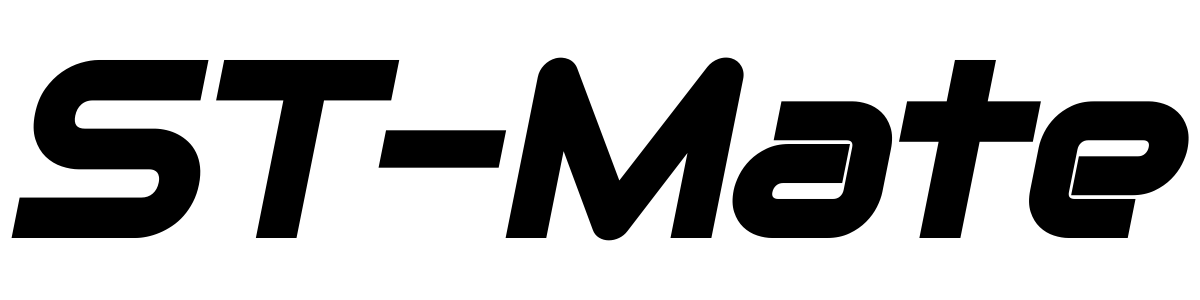
\includegraphics[width=0.6\textwidth]{logo.png}
    \end{figure}
    \vfill
    \begin{flushright}
        \textit{Разработал: А.Н. Кондратьев}\\
    \end{flushright}
    {\large \today}
\end{titlepage}

\tableofcontents

\newpage

% ========== 1 Введение ==========
\section{Введение}
\label{sec:introduction}

Настоящий документ содержит сведения, необходимые для правильной эксплуатации автоматизированной системы «ST-Mate». 
В документе приведены назначение и условия применения, подготовка к работе, описание операций действия пользователя а также рекомендации по устранению возможных нештатных ситуаций и рекомендации по освоению.

\subsection{Область применения}
«ST-Mate» предназначено для использования в качестве интеллектуальной шахматной доски для игры в классические шахматы.
Подходит для использования в домашних условиях, учебных заведениях, шахматных клубах и других местах. 

\subsection{Краткое описание возможностей средства автоматизации}
«ST-Mate» обеспечивает следующие функции:
\begin{itemize}
    \item Автоматическое распознавание положения фигур на доске.
    \item Подсветка допустимых ходов для каждой фигуры.
    \item Подсказки рекомендуемых ходов по нажатию кнопки.
    \item Управление партией в трёх режимах.
    \item Беспроводной интерфейс Bluetooth для удалённого мониторинга и управления.
\end{itemize}

\subsection{Перечень эксплуатационной документации}
К эксплуатационной документации относятся:
Руководство пользователя (настоящее руководство) - содержит информацию для пользователей о назначении, условиях применения, подготовке к работе, описании операций и рекомендациях по устранению нештатных ситуаций.

% ========== 2 Назначение и условия применения ==========
\section{Назначение и условия применения}
\label{sec:purpose}

\subsection{Назначение ST-Mate}
«ST-Mate» представляет собой интеллектуальную шахматную доску, предназначенную для игры в классические шахматы в трёх режимах:
\begin{itemize}
    \item Игрок за белые фигуры против встроенного программного движка;
    \item Игра двух игроков друг против друга без участия программного движка.
    \item Игрок за чёрные фигуры против встроенного программного движка;
\end{itemize}

«ST-Mate» обеспечивает автоматическое распознавание положения фигур на доске, подсветку допустимых ходов, подсказки и управление партией.

\subsection{Технические характеристики}

\begin{itemize}
    \item Габаритные размеры (Д×Ш×В): 455×455×45 мм.
    \item Размер игрового поля: 400×400 мм.
    \item Размер клетки: 50×50 мм.
    \item Разъём питания: USB Type-C.
    \item Напряжение питания: 5 В,
    \item Максимальный ток потребления: 500 мА.
    \item Микроконтроллер: STM32F103C8T6.
    \item Датчики положения фигур: 64 датчика Холла SS49E.
    \item Подсветка полей: адресная светодиодная лента WS2813.
    \item Шахматный движок: micro-Max версии 4.8 от H.G. Muller.
    \item Беспроводной интерфейс: Bluetooth, имя устройства «ST-Mate».
\end{itemize}

\subsection{Условия эксплуатации}
Шахматная доска «ST-Mate» предназначена для эксплуатации при температуре от +5 до +30 °C и относительной влажности не более 80 \% без конденсации.
Не допускается воздействие прямых солнечных лучей, вибрации, ударов, попадания жидкости.

% ========== 3 Подготовка к работе ==========
\section{Подготовка к работе}
\label{sec:preparation}

\subsection{Распаковка и осмотр}
Извлеките Шахматную доску «ST-Mate» из упаковочной коробки.
Убедитесь в отсутствии видимых механических повреждений корпуса, доски и фигур.
Проверьте комплектность.

В комплект входят:
\begin{itemize}
    \item Электронная шахматная доска - 1 шт.
    \item Фигуры с магнитами (32 шт.) - 1 комплект.
    \item Руководство пользователя - 1 шт.
\end{itemize}

\subsection{Подключение к источнику питания}
Убедитесь, что источник питания (не входит в комплект) соответствует требованиям (сетевой адаптер USB 5 В / не менее 500 мА или порт USB компьютера).
Кабель USB Type-C (не входит в комплект) не должен быть повреждён, разъёмы не должны иметь загрязнений или деформаций.\\
При первом включении необходимо выполнить следующие действия без наличия фигур на доске:
\begin{enumerate}
    \item Подключите конец кабеля к источнику питания.
    \item Другой конец кабеля USB Type-C подключите к разъёму на задней панели ST-Mate.
    \item После подачи питания Шахматная доска «ST-Mate» выполняет самотестирование и калибровку: кратковременно загораются все светодиоды подсветки, после чего доска переходит в режим ожидания начальной расстановки фигур.
\end{enumerate}

\subsection{Порядок проверки работоспособности}
После подключения к питанию и выполнения самотестирования убедитесь в следующем:
\begin{enumerate}
    \item Разверните доску так, чтобы ближайшее угловое поле справа от каждого игрока было белым.
    \item Первые две горизонтали (ряды 1 и 2) со стороны белых и две горизонтали (ряды 7 и 8) со стороны чёрных должны мигать красным цветом.
    \item Поля, на которых фигуры установлены, подсвечиваются зелёным цветом.
    \item Ряды 3–6 не подсвечиваются если на них нет фигур. Иначе подсвечиваются мигающим красным цветом. См. раздел \ref{sec:initial-position} \nameref{sec:initial-position}.
    \item Если белые фигуры и чёрные фигуры были установлены не на свои места (Перепутаны стороны), подсвечиваются красным мигающим светом. См. раздел \ref{sec:initial-position} \nameref{sec:initial-position}.
\end{enumerate}
В случае несоответствия вышеуказанным условиям выполните сброс кнопкой «RESET» и повторите процедуру проверки.
Если проблема сохраняется, обратитесь к разделу \ref{sec:troubleshooting} \nameref{sec:troubleshooting}.


% ========== 4 Описание операций ==========
\section{Описание операций}
\label{sec:operations}

\subsection{Органы управления}
На лицевой панели расположены (слева направо):
\begin{enumerate}
    \item Логотип.
    \item Кнопка \textbf{«HINT»} - при нажатии показывает рекомендуемый ход для стороны, которая должна совершить ход.
    \item Переключатель - имеет 3 положения, соответствующие режимам игры.
    \item Кнопка \textbf{«RNG»} (random number generator) - активирует режим, в котором движок будет выполнять случайные ходы (полезно для обучения).
\end{enumerate}
На обратной стороне доски расположены (слева направо):
\begin{enumerate}
    \item Кнопка \textbf{RESET} - принудительная перезагрузка микроконтроллера.
    \item Разъём питания \textbf{USB}.
\end{enumerate}

\subsection{Выбор режима игры}
Переключатель расположен на лицевой панели Шахматной доски «ST-Mate». 

Режимы:
\begin{itemize}
    \item \textbf{WvE} - игрок управляет белыми фигурами, ход чёрных делает контроллер.
    \item \textbf{PvP} - оба участника делают ходы поочерёдно, контроллер только отслеживает положение фигур и предоставляет подсказки.
    \item \textbf{BvE} - игрок управляет чёрными фигурами, ход белых делает контроллер.
\end{itemize}
При смене режима тумблером игра автоматически сбрасывается. Для начала новой игры необходимо установить фигуры в начальное положение (см. раздел \ref{sec:initial-position} \nameref{sec:initial-position}).

После установки фигур и выбора режима Шахматная доска «ST-Mate» готова к игре.

\subsection{Начальное положение фигур}
\label{sec:initial-position}
Перед началом игры необходимо установить фигуры в начальное положение, соответствующее стандартной шахматной стартовой позиции (рис. \ref{fig:startpos}). 
Фигуры распознаются автоматически с помощью встроенных датчиков Холла. 

\begin{figure}[H]
    \centering
    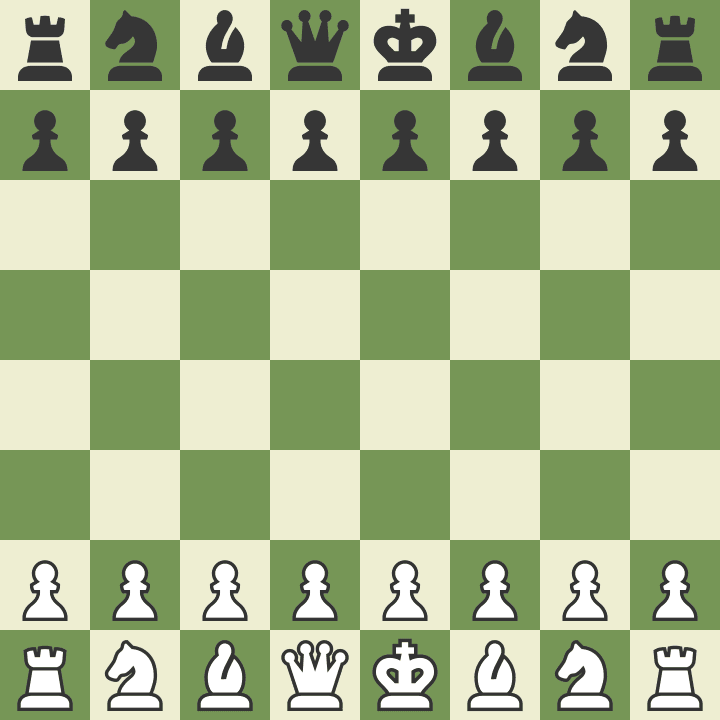
\includegraphics[width=0.5\textwidth]{chess position.png}
    \caption{Начальное положение фигур на доске}
    \label{fig:startpos}
\end{figure}

\textbf{Важно:} после каждого переключения режима игры или при включении питания доска автоматически переходит в состояние ожидания начальной расстановки. 
Фигуры должны быть установлены на свои места вручную. После завершения расстановки контроллер автоматически распознаёт все фигуры и готов к игре.


\subsection{Порядок выполнения хода}
По правилам шахмат игроки поочередно выполняют ходы. Белые ходят первыми.
Процесс выполнения хода включает следующие шаги:
\begin{enumerate}
    \item Игрок, чья очередь хода, берёт фигуру своего цвета и ставит её на поле назначения. Датчики Холла фиксируют изменение положения фигур.
    \item Если ход выполнен в соответствии с правилами шахмат, контроллер подтверждает его подсветкой полей. Ход считается сделанным, очередь переходит сопернику (или контроллеру).
    \item При попытке выполнить недопустимый ход (например, на поле, недоступное для фигуры, или под шах) подсветка полей становится красной, ход не принимается. Игрок должен вернуть фигуру на исходное поле и выбрать другой ход.
\end{enumerate}

Взятие фигуры включает следующие шаги:
\begin{enumerate}
    \item Игрок, чья очередь хода, берёт фигуру своего цвета.
    \item Фигуру противника игрок также берёт в свою руку.
    \item Игрок ставит свою фигуру на место фигуры противника. 
\end{enumerate}
Если взятие выполнено в соответствии с правилами шахмат, контроллер подтверждает ход подсветкой совершенного хода.

\subsection{Особые ходы}
\textbf{Рокировка:} особый ход заключающийся в горизонтальном перемещении короля в сторону ладьи своего цвета на 2 клетки и последующем перемещении ладьи на соседнюю с королём клетку по другую сторону от короля.
Каждая из сторон может сделать одну рокировку в течение партии.

Процесс рокировки на королевский фланг изображён на рис. \ref{fig:kingside castling}.
\begin{figure}[H]
    \centering
    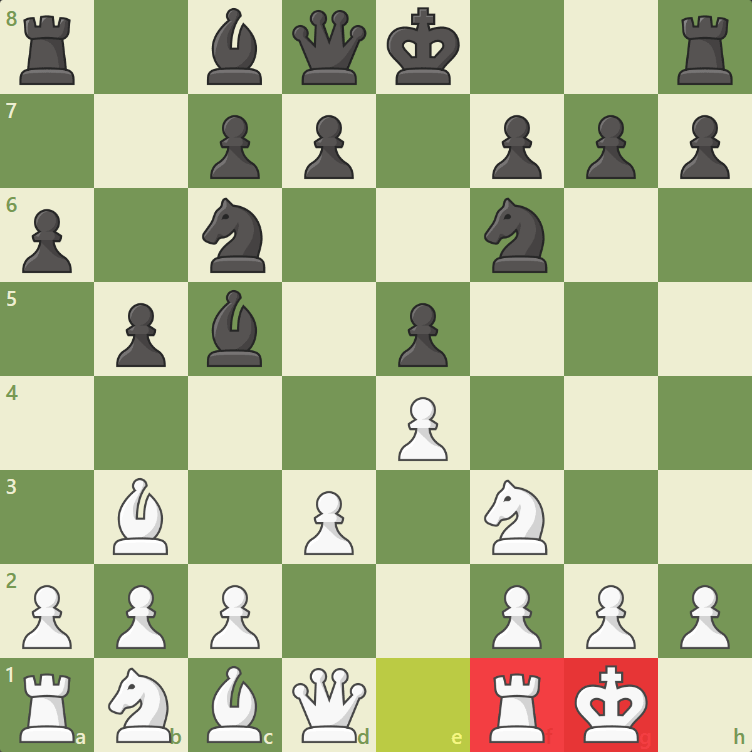
\includegraphics[width=0.4\textwidth]{kingside castling.png}
    \caption{Рокировка на королевский фланг}
    \label{fig:kingside castling}
\end{figure}

Процесс рокировки на ферзевый фланг изображён на рис. \ref{fig:queenside castling}.
\begin{figure}[H]
    \centering
    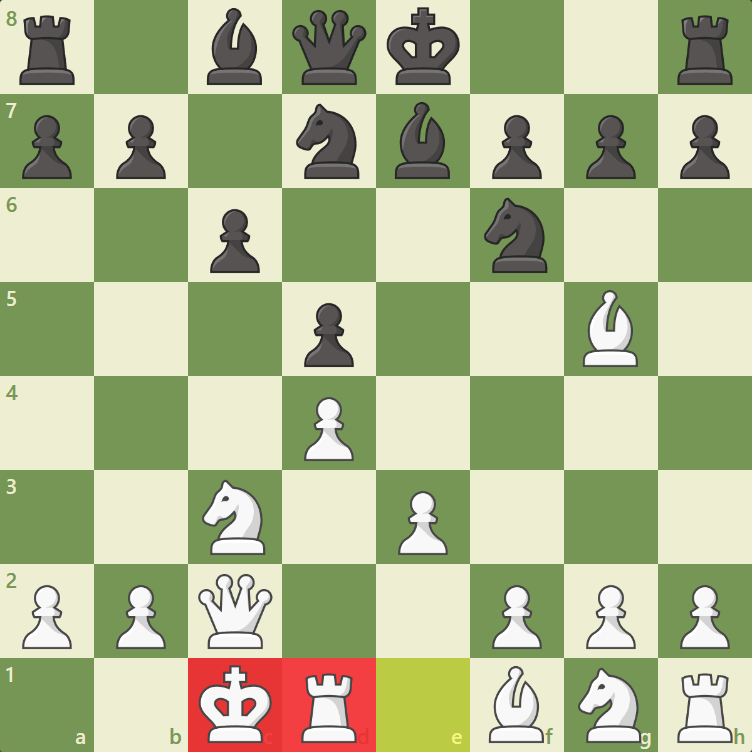
\includegraphics[width=0.4\textwidth]{queenside castling.png}
    \caption{Рокировка на ферзевый фланг}
    \label{fig:queenside castling}

\end{figure}

Процесс выполнения рокировки включает следующие шаги:
\begin{enumerate}
    \item Игрок, чья очередь хода, берёт короля своего цвета и ставит на поле назначения.
    \item Следом переносит ладью своего цвета на соседнюю клетку по другую сторону от короля.
    \item Процесс выполнения рокировки будет указывать на положение короля и ладьи.
    \item Если ход выполнен в соответствии с правилами шахмат, контроллер подтверждает его подсветкой полей. Ход считается сделанным, очередь переходит сопернику (или контроллеру).
    \item При попытке выполнить недопустимый ход (например, на поле, недоступное для фигуры или под шах) подсветка полей становится красным, ход не принимается. Игрок должен вернуть фигуру на исходное поле и выбрать другой ход.
\end{enumerate}

\textbf{Взятие на проходе:} особый ход пешки  при котором она берёт пешку противника, перемещённую с начальной позиции сразу на два поля. При взятии на проходе под боем оказывается не то поле, на котором остановилась вторая пешка, а то, которое было пересечено ею. Первая пешка завершает взятие именно на этом, пересечённом поле, как если бы пешка противника переместилась лишь на одно поле. Взятие возможно только ходом, следующим за продвижением пешки противника.

Процесс взятия на проходе изображён на рис. \ref{fig:en passant}.
\begin{figure}[H]
    \centering
    \includegraphics[width=0.4\textwidth]{en passant.png}
    \caption{Взятие на проходе}
    \label{fig:en passant}
\end{figure}

Процесс взятия на проходе включает следующие шаги:
\begin{enumerate}
    \item Игрок, чья очередь хода, берёт пешку своего цвета.
    \item Следом берёт пешку противника и удаляет её с доски.
    \item Ставит свою пешку на поле, пересечённое пешкой противника.
    \item Если ход выполнен в соответствии с правилами шахмат, контроллер подтверждает его подсветкой полей. Ход считается сделанным, очередь переходит сопернику (или контроллеру).
    \item При попытке выполнить недопустимый ход (например, на поле, недоступное для фигуры) подсветка полей становиься красным, ход не принимается. Игрок должен вернуть фигуру на исходное поле и выбрать другой ход.
\end{enumerate}

\textbf{Превращение:} особый ход заключающийся в превращение пешки, дошедшей до последнего ряда в другую фигуру. 
В текущей версии программного обеспечения пешка автоматически превращается в ферзя. Возможность выбора фигуры будет добавлена в следующих обновлениях.

Процесс выполнения превращения включает следующие шаги:
\begin{enumerate}
    \item Игрок, чья очередь хода, берёт пешку своего цвета на предпоследнем ряду.
    \item Меняет её на Ферзя своего цвета и ставит на поле назначения.
    \item В случае если доступно взятие фигуры противника на последней диагонали игрок делает взятие, и ставит на поле взятия Ферзя.
    \item Если ход выполнен в соответствии с правилами шахмат, контроллер подтверждает его подсветкой полей. Ход считается сделанным, очередь переходит сопернику (или контроллеру).
    \item При попытке выполнить недопустимый ход (например, на поле, недоступное для фигуры) подсветка полей становится красным, ход не принимается. Игрок должен вернуть фигуру на исходное поле и выбрать другой ход.
\end{enumerate}

\subsection{Использование кнопки HINT}
На боковой панели Шахматной доски «ST-Mate» расположена кнопка «HINT».
Подсказка не влияет на очередность хода и не совершает ход автоматически.

\subsection{Использование кнопки RNG}
На боковой панели Шахматной доски «ST-Mate» расположена кнопка «RNG».
Кнопка RNG предназначена для включения генерации случайного хода контроллера в режимах с участием программного движка.
Активация режима RNG возможна только при включении доски или при перезагрузке.

\subsection{Сброс и перезагрузка}
При необходимости принудительного сброса Шахматной доски «ST-Mate» (например, при зависании или для начала новой партии) используйте кнопку «RESET», расположенную рядом с разъёмом USB Type-C. 
Короткое нажатие кнопки приводит к перезагрузке микроконтроллера и повторному выполнению процедуры инициализации. 
После перезагрузки требуется заново установить фигуры в начальное положение.

\subsection{Управление по Bluetooth}
Для удалённого управления и мониторинга доска оснащена Bluetooth-интерфейсом. 
Подключитесь к нему с помощью смартфона, планшета или компьютера, используя любой терминальный клиент (например, \textit{Serial Bluetooth Terminal}).
После подключения доступен текстовый протокол команд. 
Команды передаются в кодировке UTF-8, заканчиваются символом \texttt{\textbackslash{r}\textbackslash{n}} (возврат каретки и перевод строки).

\subsection{Подключение}
При запуске Шахматной доски «ST-Mate» она становится доступной для подключения по Bluetooth под именем \texttt{ST-Mate}.

% ========== Аварийные ситуации ==========
\section{Аварийные ситуации}
\label{sec:troubleshooting}

В таблице \ref{tab:errors} приведены возможные нештатные ситуации и рекомендации по их устранению.
\begin{table}[H]
    \centering
    \begin{tabular}{|p{0.3\textwidth}|p{0.6\textwidth}|}
        \hline
        \textbf{Ситуация} & \textbf{Действия пользователя} \\
        \hline
        Шахматная доска «ST-Mate» не включается, подсветка отсутствует & 
        Проверить подключение кабеля USB Type-C, убедиться, что источник питания обеспечивает напряжение 5 В и ток не менее 500 мА.
        Попробовать другой кабель или порт USB. \\
        \hline
        Фигуры не распознаются (нет реакции на перемещение) & 
        Убедиться, что фигуры используются из оригинального набора и установлены строго в центре полей. 
        При необходимости выполнить сброс кнопкой «RESET» и заново расставить фигуры. \\
        \hline
        Некорректная подсветка (мигание хаотичное) & 
        Возможно воздействие внешних магнитных полей. 
        Удалить источники сильных магнитных полей. 
        Выполнить перезагрузку. \\
        \hline
        Подсветка фигур не соответствует их расположению &
        Увеличить уровень срабатывания датчиков в настройках на 5–10 единиц.
        Увеличить коэффициент сглаживания в настройках на 1–2 единиц.
        Проверить блок питания на соответствие требованиям.
        Уменьшить яркость подсветки в настройках. \\
        \hline
        После калибровки датчики не реагируют на фигуры & 
        Убедиться, что калибровка выполнялась при отсутствии фигур на доске. 
        Выполнить принудительную калибровку повторно. 
        Поменять значения уровня срабатывания и коэффициент сглаживания. \\
        \hline
        Программа не делает ход в режимах с контроллером & 
        Проверить, что режим выбран корректно и очередь хода принадлежит контроллеру. 
        Если задержка превышает 10 секунд, нажать кнопку «HINT» для инициирования хода. \\
        \hline
        Не работает Bluetooth, нет ST-Mate в списке устройств &
        Убедиться, что ST-Mate включен. Обратиться к разработчику ST-Mate. \\
        \hline
    \end{tabular}
    \caption{Нештатные ситуации и способы их устранения}
    \label{tab:errors}
\end{table}

% ========== Рекомендации по освоению ==========
\section{Рекомендации по освоению}
\label{sec:usage}
Для быстрого освоения Шахматной доски «ST-Mate» рекомендуется:
\begin{itemize}
    \item Внимательно ознакомиться с данным руководством, особенно с разделами \ref{sec:operations} \nameref{sec:operations} и \ref{sec:troubleshooting} \nameref{sec:troubleshooting}.
    \item Ознакомиться с правилами игры в шахматы ФИДЕ. Ссылка на официальный справочник ФИДЕ: \url{https://handbook.fide.com/} (дата обращения: 01.04.2026).
    \item Начать с режима «игрок против игрока» без использования подсказок, чтобы привыкнуть к физическому взаимодействию с доской и понять принцип распознавания ходов.
    \item После освоения базовых операций перейти к игре против контроллера, используя подсказки для изучения тактических приёмов.
    \item При возникновении сомнений в корректности положения фигур пользоваться кнопкой «Сброс» и начинать партию заново.
\end{itemize}

\subsection{Визуальные сообщения пользователю}

Шахматная доска «ST-Mate» использует различные способы информирования пользователя о текущем состоянии и событиях.
Для освоения рекомендуется использовать стандартную цветовую тему подсветки (THEME:0), которая интуитивно отображает допустимые ходы и ошибки.
Далее будут приведены примеры световой индикации для стандартной световой темы.

Для начальной расстановки фигур и ожидания начала партии поля первого, второго ряда со стороны белых и седьмого и восьмого ряда со стороны чёрных подсвечиваются красным цветом, а центральные 4 ряда не подсвечиваются.
Как только фигуры будут установлены на свои места, доска распознает их отключит подсветку.
При выборе фигуры, поле на котором она находится, начинает мигать белым цветом. Допустимые ходы для выбранной фигуры подсвечиваются белым.
Как только фигура будет перемещена на новое поле, будет подсвечено совершённое перемещение желтым цветом. И ход передаётся сопернику (или контроллеру).
При попытке выполнить недопустимый ход, поля начнут мигать красным цветом.
При нажатии кнопки «HINT» для отображения рекомендуемого хода, поля, на которые рекомендуется ходить, будут подсвечены голубым цветом.
При рокировке поля, на которые перемещаются король будут подсвечены белым цветом. После перемещения короля будет отмечено совершённое перемещение желтым цветом. 
Далее следует перемещение ладьи, которая будет подсвечиваться белым цветом. После перемещения ладьи ход будет передан сопернику (или контроллеру).
При совершении шаха атакующая фигура будет мигать синим цветом, а король, находящийся под шахом, будет мигать красным цветом.
При совершении мата атакующая фигура будет мигать зелёным цветом, а король, находящийся под матом, будет мигать красным цветом. Игра будет завершена.
При патовой ситуации короли будут мигать жёлтым цветом. Игра будет завершена.
После окончания партии, любое перемещение фигуры приведёт к ожиданию начальной расстановки для новой партии, и поля первого, второго ряда со стороны белых и седьмого и восьмого ряда со стороны чёрных снова подсветятся красным цветом.

\subsection{Текстовые сообщения пользователю по Bluetooth}
Использование Bluetooth для получения подробной информации о ходах и состоянии партии может быть полезно для анализа и обучения, но не является обязательным для базовой эксплуатации.
По интерфейсу Bluetooth ST-Mate может отправлять текстовые сообщения, информируя пользователя о текущем состоянии, результатах ходов и других событиях.
Совершенные ходы выводятся в алгебраической нотации (например, «e2e4» для хода пешки с поля e2 на поле e4).
Ходы которые были отклонены из-за нарушения правил, сопровождаются сообщением об ошибке (например, «White make invalid move e2e5»).
По окончании партии выводится результат (например, «1-0» для победы белых, «0-1» для победы чёрных, «1/2-1/2» для ничьей).
Также выводится PGN текущий партии для возможности её сохранения и анализа. Вывод об инициализации, запуске, ходе игры и результате в формате PGN представлен на рис. \ref{fig:log}

\begin{figure}[H]
    \centering
    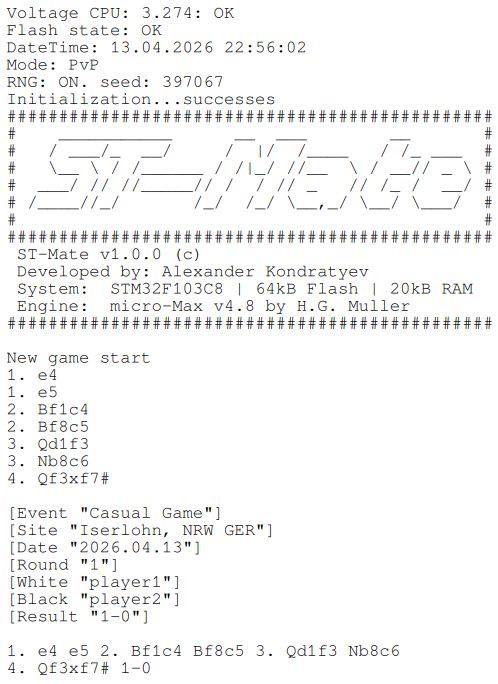
\includegraphics[width=0.6\textwidth]{log.png}
    \caption{Лог сообщений по Bluetooth}
    \label{fig:log}
\end{figure}

\subsection{Отправка команд}
После подключения к доске по Bluetooth пользователь может отправлять текстовые команды. 
Команды не чувствительны к регистру.
Поддерживаемые запросы и команды в Приложении А.

\subsection{Примеры использования}
\begin{verbatim}
> BRIGHT:80\r\n 
Brightness set:80\r\n
> THEME:5\r\n
Theme set:5\r\n
> TRIGLV?\r\n
Trigger level:40\r\n
\end{verbatim}

% ========== Техническое обслуживание ==========
\section{Техническое обслуживание}
\label{sec:maintenance}

Во избежание травм и повреждений, а также для обеспечения долгого срока службы Шахматной доски «ST-Mate», рекомендуется соблюдать следующие рекомендации по техническому обслуживанию.
\begin{itemize}
    \item Не разбирайте устройство самостоятельно, так как это может привести к травмам и повреждениям.
    \item Храните доску и фигуры в чистоте, избегайте попадания жидкости внутрь корпуса.
    \item Регулярно проверяйте целостность кабеля питания и разъёма USB Type-C. Не используйте повреждённые кабели.
    \item При хранении и транспортировке используйте оригинальную упаковку или аналогичную по уровню защиты от ударов и вибраций.
    \item Не подвергайте устройство воздействию экстремальных температур, прямых солнечных лучей или сильных магнитных полей.
\end{itemize}
При возникновении неисправностей обратитесь к разделу «Аварийные ситуации» или свяжитесь с разработчиками.

\subsection{Калибровка датчиков}
Рекомендуется выполнять калибровку при первом включении, замене блока питания, кабеля или при изменении условий эксплуатации (температура, влажность). 
Калибровочная таблица сохраняется в энергонезависимой памяти.
Калибровка производится автоматически при включении или сбросе если на доске нет фигур.\\
Есть два способа выполнить принудительную калибровку:

\begin{enumerate}
    \item При зажатой кнопке «HINT» при включении питания или при нажатии кнопки «RESET».
    \item Терминальной командой \texttt{CALIBRATE\textbackslash{r}\textbackslash{n}} по Bluetooth.
\end{enumerate}

Для выполнения принудительной калибровки выполните следующие действия:
\begin{itemize}
    \item Снимите все фигуры с доски.
    \item Выполните один из способов запуска калибровки.
    \item Дождитесь завершения процесса (около 5 секунд).
\end{itemize}

\subsection{Хранение и транспортировка}
Храните Шахматную доску «ST-Mate» в сухом, чистом месте при температуре от +5 до +30 °C.
При транспортировке используйте оригинальную упаковку или аналогичную по уровню защиты от ударов и вибраций. 
Избегайте воздействия прямых солнечных лучей, влаги, экстремальных температур и механических повреждений.

\subsection{Уход за поверхностью}
Протирайте корпус и фигуры мягкой слегка влажной тканью. Не допускайте попадания жидкости внутрь корпуса. Не используйте абразивные чистящие средства.


\newpage
% ========== Перечень принятых сокращений ==========
\section{Перечень принятых сокращений}
\label{sec:abbreviations}

\begin{itemize}
    \item АС - автоматизированная система.
    \item USB - универсальная последовательная шина (Universal Serial Bus).
    \item LED - светоизлучающий диод (Light Emitting Diode).
    \item Bluetooth - беспроводная технология обмена данными на коротких расстояниях.
    \item PGN - Portable Game Notation, формат записи шахматных партий.
    \item FEN - Forsyth-Edwards Notation, формат описания позиции в шахматах.
    \item RNG - генератор случайных чисел (Random Number Generator).
    \item STM32 - семейство 32-битных микроконтроллеров от STMicroelectronics.
    \item SS49E - датчик Холла, используемый для определения наличия магнитного поля.
    \item WS2813 - тип адресной светодиодной ленты.
    \item micro-Max - компактный шахматный движок, разработанный H.G. Muller. Исходный код доступен по ссылке: \url{https://home.hccnet.nl/h.g.muller/umax4_8.c} (дата обращения: 01.04.2026).
\end{itemize}

\newpage

% ========== Сведения о разработчиках и контактная информация ==========
\section{Сведения о разработчиках и контактная информация}
\label{sec:developers}

\begin{itemize}
    \item \textbf{Разработчик шахматной доски ST-Mate:} Кондратьев Александр Николаевич.\\
          Email: \texttt{alexander.kondratyev.dev@gmail.com}\\
          Telegram: \url{https://t.me/kondratyev_an}
    \item \textbf{Разработчик шахматного движка micro-Max:} H.G. Muller.\\
          Домашняя страница: \url{https://home.hccnet.nl/h.g.muller/} (дата обращения: 01.04.2026).
\end{itemize}
Все вопросы по эксплуатации, настройке и доработке Шахматной доски «ST-Mate» направлять разработчикам.

\newpage

% ========== ПРИЛОЖЕНИЯ ==========
\clearpage
\section*{Приложение А. Протокол команд}
\addcontentsline{toc}{section}{Приложение А. Протокол команд}
\label{sec:protocol}

\begin{longtable}{|p{0.15\textwidth}|p{0.80\textwidth}|}
\hline
\textbf{Команда} & \textbf{Описание} \\ \hline
\endfirsthead
\hline
\textbf{Команда} & \textbf{Описание} \\ \hline
\endhead
\hline
\endfoot
\multicolumn{2}{|c|}{\textbf{Служебные}} \\ \hline
\texttt{REBOOT} & Перезагрузка устройства (аналог нажатия кнопки RESET). \\ \hline
\texttt{SERVICE:X} & Включение/выключение сервисного режима. X=0 - выключен, X=1 - включён. \\ \hline
\texttt{VOLT?} & Запрос напряжения питания процессора (возвращает значение в милливольтах). \\ \hline
\texttt{CALIBRATE} & Запуск калибровки датчиков (доска должна быть пустой). \\ \hline
\texttt{TRIGLV?} & Запрос текущего уровня срабатывания датчиков (по умолчанию 25). \\ \hline
\texttt{TRIGLV:X} & Установка уровня срабатывания датчиков (X - целое число, зависящее от калибровки). \\ \hline
\texttt{ALPHA?} & Запрос текущего значения коэффициента экспоненциального сглаживания (по умолчанию 8). \\ \hline
\texttt{ALPHA:X} & Установка коэффициента экспоненциального сглаживания (X - целое число). \\ \hline
\multicolumn{2}{|c|}{\textbf{Пользовательские}} \\ \hline
\texttt{EVENT?} & Запрос названия турнира, матча. \\ \hline
\texttt{EVENT:X} & Установка названия турнира, матча. (например: EVENT:Casual Game). \\ \hline
\texttt{SITE?} & Запрос места проведения. \\ \hline
\texttt{SITE:X} & Установка места проведения. (например: SITE:Moscow). \\ \hline
\texttt{TIME?} & Запрос текущего времени \\ \hline
\texttt{TIME:X} & Установка текущего времени (X - строка в формате dd.mm.yy HH:MM:SS). \\ \hline
\texttt{ROUND?} & Запрос номера раунда. \\ \hline
\texttt{ROUND:X} & Установка номера раунда. (например: ROUND:1). \\ \hline
\texttt{WHITE?} & Запрос имени игрока за белые фигуры. \\ \hline
\texttt{WHITE:X} & Установка имени игрока за белые фигуры. (например: WHITE:Alice). \\ \hline
\texttt{BLACK?} & Запрос имени игрока за чёрные фигуры. \\ \hline
\texttt{BLACK:X} & Установка имени игрока за чёрные фигуры. (например: BLACK:Bob). \\ \hline
\texttt{FEN?} & Запрос текущей позиции в формате FEN. \\ \hline
\texttt{PGN?} & Запрос текущей партии в формате PGN. \\ \hline
\texttt{SEED?} & Запрос текущего зерна для генератора случайных чисел. \\ \hline
\texttt{SEED:X} & Установка зерна для генератора случайных чисел (X - целое число или строка). \\ \hline
\texttt{BRIGHT?} & Запрос текущего уровня яркости подсветки. \\ \hline
\texttt{BRIGHT:X} & Установка яркости подсветки (0–100). Пример:\texttt{BRIGHT:50}. \\ \hline
\texttt{THEME:X} & Установка цветовой темы (0–11). Перечень тем приведён в \nameref{sec:themes}. \\ \hline
\texttt{HINTBTN:X} & Включение/выключение кнопки подсказки. X=0 - кнопка неактивна, X=1 - активна. \\ \hline
\end{longtable}

\clearpage
\section*{Приложение Б. Цветовые схемы подсветки}
\addcontentsline{toc}{section}{Приложение Б. Цветовые схемы подсветки}
\label{sec:themes}

\begin{center}
\begin{tabular}{|c|l|}
\hline
\textbf{Код} & \textbf{Название темы} \\ \hline
    0 & Default - стандартная тема (по умолчанию) \\
    1 & Neon Night - яркие неоновые цвета \\
    2 & Forest Glade - природные зеленые и коричневые оттенки \\
    3 & Ocean Breeze - морская тема с синими тонами \\
    4 & Royal Purple - благородные фиолетовые оттенки \\
    5 & Autumn Sunset - теплые осенние цвета \\
    6 & Arctic Ice - холодные пастельные тона \\
    7 & Desert Sand - песочные и земляные оттенки \\
    8 & Candy Land - яркие конфетные цвета \\
    9 & Midnight Oil - темные насыщенные тона \\
    10 & Spring Meadow - свежие весенние цвета \\
    11 & Classic Elegance - сдержанная классическая гамма \\
\hline
\end{tabular}
\end{center}

\end{document}
